\documentclass[tikz,border=5pt]{standalone}
\usepackage{tikz}
\usetikzlibrary{positioning,shapes.geometric,arrows.meta,fit,calc}

\definecolor{inputcolor}{RGB}{240,240,240}
\definecolor{backbonecolor}{RGB}{232,245,232}
\definecolor{densecolor}{RGB}{227,242,253}
\definecolor{attentioncolor}{RGB}{243,229,245}
\definecolor{fusioncolor}{RGB}{255,243,224}

\begin{document}
	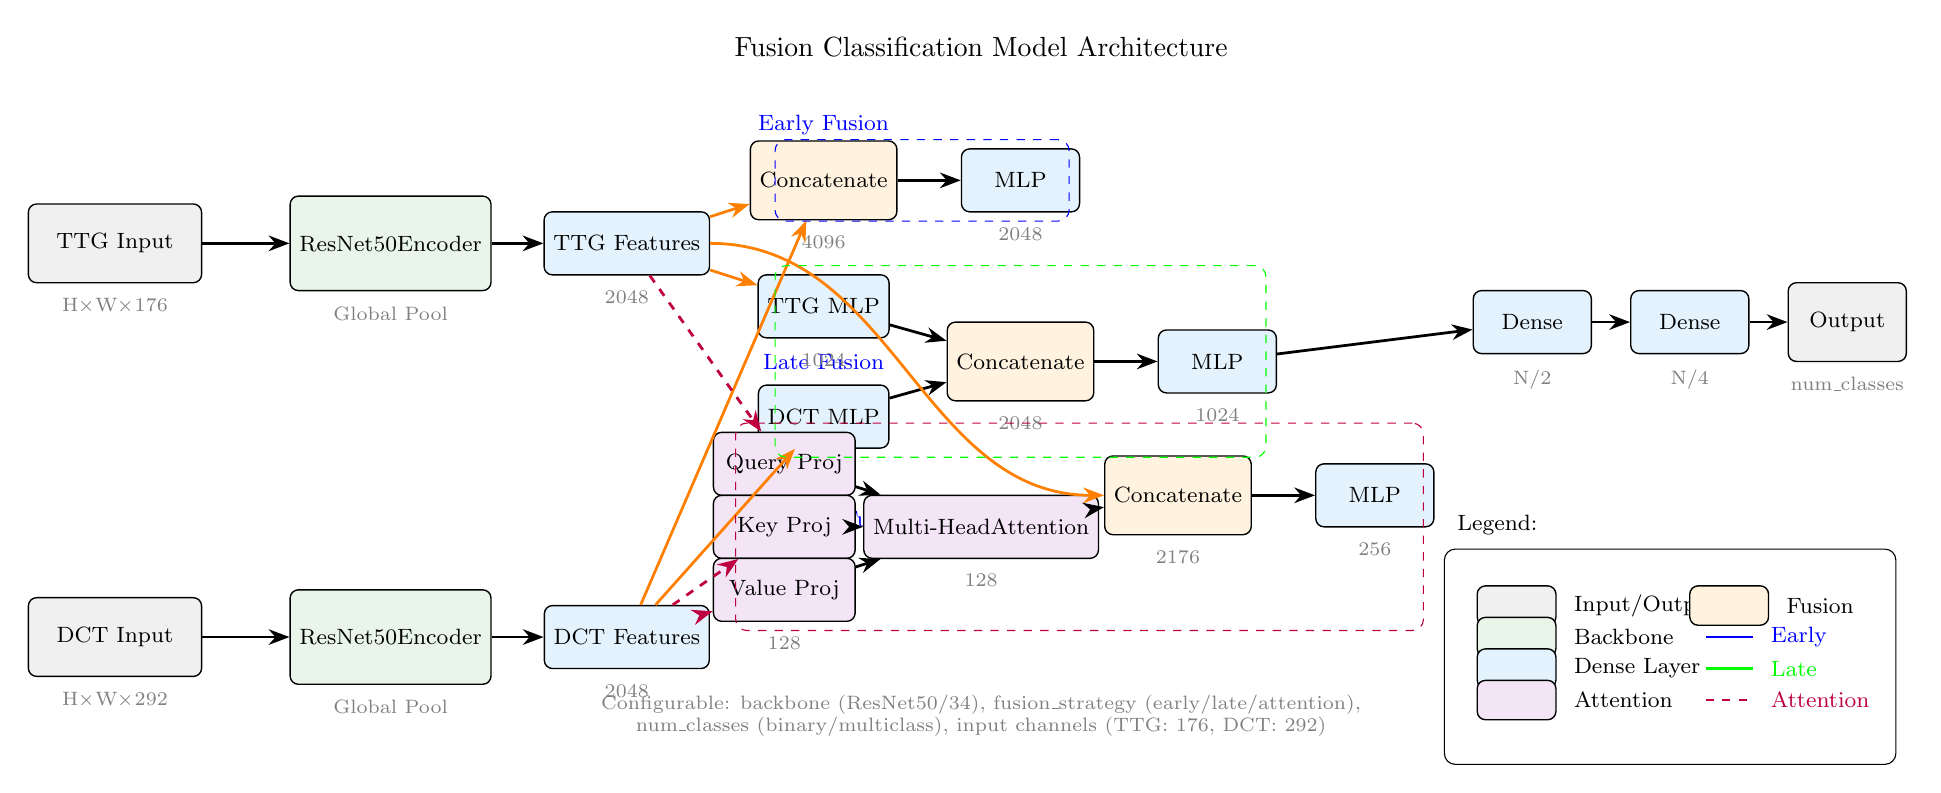
\begin{tikzpicture}[
		% Layer styles
		input/.style={rectangle, rounded corners=3pt, minimum height=1cm, minimum width=2.2cm, 
			fill=inputcolor, draw=black, line width=0.5pt, text centered, font=\footnotesize},
		backbone/.style={rectangle, rounded corners=3pt, minimum height=1.2cm, minimum width=2cm,
			fill=backbonecolor, draw=black, line width=0.5pt, text centered, font=\footnotesize},
		dense/.style={rectangle, rounded corners=3pt, minimum height=0.8cm, minimum width=1.5cm,
			fill=densecolor, draw=black, line width=0.5pt, text centered, font=\footnotesize},
		attention/.style={rectangle, rounded corners=3pt, minimum height=0.8cm, minimum width=1.8cm,
			fill=attentioncolor, draw=black, line width=0.5pt, text centered, font=\footnotesize},
		fusion/.style={rectangle, rounded corners=3pt, minimum height=1cm, minimum width=1.8cm,
			fill=fusioncolor, draw=black, line width=0.5pt, text centered, font=\footnotesize},
		output/.style={rectangle, rounded corners=3pt, minimum height=1cm, minimum width=1.5cm,
			fill=inputcolor, draw=black, line width=0.5pt, text centered, font=\footnotesize},
		% Arrow styles
		arrow/.style={->, >=Stealth, thick, line width=1pt},
		fusionarrow/.style={->, >=Stealth, thick, line width=1pt, color=orange},
		attnarrow/.style={->, >=Stealth, thick, line width=1pt, dashed, color=purple},
		% Text styles
		dimlabel/.style={font=\scriptsize, text=gray},
		layerlabel/.style={font=\footnotesize},
		strategylabel/.style={font=\footnotesize, color=blue}
		]
		
		% Input layers
		\node[input] (ttg_input) at (0,6) {TTG Input};
		\node[dimlabel, below=2pt of ttg_input] {H×W×176};
		
		\node[input] (dct_input) at (0,1) {DCT Input};
		\node[dimlabel, below=2pt of dct_input] {H×W×292};
		
		% Backbone encoders
		\node[backbone] (ttg_encoder) at (3.5,6) {ResNet50\\Encoder};
		\node[dimlabel, below=2pt of ttg_encoder] {Global Pool};
		
		\node[backbone] (dct_encoder) at (3.5,1) {ResNet50\\Encoder};
		\node[dimlabel, below=2pt of dct_encoder] {Global Pool};
		
		% Feature extraction
		\node[dense] (ttg_features) at (6.5,6) {TTG Features};
		\node[dimlabel, below=2pt of ttg_features] {2048};
		
		\node[dense] (dct_features) at (6.5,1) {DCT Features};
		\node[dimlabel, below=2pt of dct_features] {2048};
		
		% Strategy 1: Early Fusion
		\node[strategylabel] at (9,7.5) {Early Fusion};
		\node[fusion] (early_concat) at (9,6.8) {Concatenate};
		\node[dimlabel, below=2pt of early_concat] {4096};
		\node[dense] (early_mlp) at (11.5,6.8) {MLP};
		\node[dimlabel, below=2pt of early_mlp] {2048};
		
		% Strategy 2: Late Fusion
		\node[strategylabel] at (9,4.5) {Late Fusion};
		\node[dense] (ttg_mlp) at (9,5.2) {TTG MLP};
		\node[dimlabel, below=2pt of ttg_mlp] {1024};
		\node[dense] (dct_mlp) at (9,3.8) {DCT MLP};
		\node[dimlabel, below=2pt of dct_mlp] {1024};
		\node[fusion] (late_concat) at (11.5,4.5) {Concatenate};
		\node[dimlabel, below=2pt of late_concat] {2048};
		\node[dense] (late_mlp) at (14,4.5) {MLP};
		\node[dimlabel, below=2pt of late_mlp] {1024};
		
		% Strategy 3: Attention Fusion
		\node[strategylabel] at (9,2.5) {Attention Fusion};
		\node[attention] (query_proj) at (8.5,3.2) {Query Proj};
		\node[dimlabel, below=2pt of query_proj] {128};
		\node[attention] (key_proj) at (8.5,2.4) {Key Proj};
		\node[dimlabel, below=2pt of key_proj] {128};
		\node[attention] (value_proj) at (8.5,1.6) {Value Proj};
		\node[dimlabel, below=2pt of value_proj] {128};
		\node[attention] (multihead_attn) at (11,2.4) {Multi-Head\\Attention};
		\node[dimlabel, below=2pt of multihead_attn] {128};
		\node[fusion] (attn_concat) at (13.5,2.8) {Concatenate};
		\node[dimlabel, below=2pt of attn_concat] {2176};
		\node[dense] (attn_mlp) at (16,2.8) {MLP};
		\node[dimlabel, below=2pt of attn_mlp] {256};
		
		% Final classifier (shared)
		\node[dense] (classifier1) at (18,5) {Dense};
		\node[dimlabel, below=2pt of classifier1] {N/2};
		\node[dense] (classifier2) at (20,5) {Dense};
		\node[dimlabel, below=2pt of classifier2] {N/4};
		\node[output] (final_output) at (22,5) {Output};
		\node[dimlabel, below=2pt of final_output] {num\_classes};
		
		% Input arrows
		\draw[arrow] (ttg_input) -- (ttg_encoder);
		\draw[arrow] (dct_input) -- (dct_encoder);
		\draw[arrow] (ttg_encoder) -- (ttg_features);
		\draw[arrow] (dct_encoder) -- (dct_features);
		
		% Early fusion arrows
		\draw[fusionarrow] (ttg_features) -- (early_concat);
		\draw[fusionarrow] (dct_features) -- (early_concat);
		\draw[arrow] (early_concat) -- (early_mlp);
		
		% Late fusion arrows
		\draw[fusionarrow] (ttg_features) -- (ttg_mlp);
		\draw[fusionarrow] (dct_features) -- (dct_mlp);
		\draw[arrow] (ttg_mlp) -- (late_concat);
		\draw[arrow] (dct_mlp) -- (late_concat);
		\draw[arrow] (late_concat) -- (late_mlp);
		
		% Attention fusion arrows
		\draw[attnarrow] (ttg_features) -- (query_proj);
		\draw[attnarrow] (dct_features) -- (key_proj);
		\draw[attnarrow] (dct_features) -- (value_proj);
		\draw[arrow] (query_proj) -- (multihead_attn);
		\draw[arrow] (key_proj) -- (multihead_attn);
		\draw[arrow] (value_proj) -- (multihead_attn);
		\draw[fusionarrow] (ttg_features.east) to[out=0,in=180] (attn_concat.west);
		\draw[arrow] (multihead_attn) -- (attn_concat);
		\draw[arrow] (attn_concat) -- (attn_mlp);
		
		% Final classification arrows (示例连接到late fusion)
		\draw[arrow] (late_mlp) -- (classifier1);
		\draw[arrow] (classifier1) -- (classifier2);
		\draw[arrow] (classifier2) -- (final_output);
		
		% Strategy selection indication
		\node[draw, dashed, rounded corners, fit={(8.5,6.4) (12,7.2)}, color=blue] (early_box) {};
		\node[draw, dashed, rounded corners, fit={(8.5,3.4) (14.5,5.6)}, color=green] (late_box) {};
		\node[draw, dashed, rounded corners, fit={(8,1.2) (16.5,3.6)}, color=purple] (attn_box) {};
		
		% Legend
		\node[draw, rounded corners, fit={(17,-0.5) (22.5,2)}, fill=white] (legend) {};
		\node[layerlabel, above right=2pt of legend.north west] {Legend:};
		\node[input, minimum width=1cm, minimum height=0.5cm] at (17.8,1.4) {};
		\node[layerlabel, right=3pt] at (18.3,1.4) {Input/Output};
		\node[backbone, minimum width=1cm, minimum height=0.5cm] at (17.8,1.0) {};
		\node[layerlabel, right=3pt] at (18.3,1.0) {Backbone};
		\node[dense, minimum width=1cm, minimum height=0.5cm] at (17.8,0.6) {};
		\node[layerlabel, right=3pt] at (18.3,0.6) {Dense Layer};
		\node[attention, minimum width=1cm, minimum height=0.5cm] at (17.8,0.2) {};
		\node[layerlabel, right=3pt] at (18.3,0.2) {Attention};
		\node[fusion, minimum width=1cm, minimum height=0.5cm] at (20.5,1.4) {};
		\node[layerlabel, right=3pt] at (21,1.4) {Fusion};
		
		% Strategy labels
		\draw[color=blue, line width=1pt] (20.2,1.0) -- (20.8,1.0);
		\node[layerlabel, right=3pt, color=blue] at (20.8,1.0) {Early};
		\draw[color=green, line width=1pt] (20.2,0.6) -- (20.8,0.6);
		\node[layerlabel, right=3pt, color=green] at (20.8,0.6) {Late};
		\draw[color=purple, line width=1pt, dashed] (20.2,0.2) -- (20.8,0.2);
		\node[layerlabel, right=3pt, color=purple] at (20.8,0.2) {Attention};
		
		% Title
		\node[layerlabel, font=\normalsize] at (11,8.5) {Fusion Classification Model Architecture};
		
		% Configuration notes
		\node[layerlabel, font=\scriptsize, text=gray] at (11,0) {
			\begin{tabular}{c}
				Configurable: backbone (ResNet50/34), fusion\_strategy (early/late/attention), \\
				num\_classes (binary/multiclass), input channels (TTG: 176, DCT: 292)
		\end{tabular}};
		
	\end{tikzpicture}
\end{document}